% vim: set tw=78 sts=2 sw=2 ts=8 aw et ai:
\documentclass{workshop}

% Comentează liniile de mai jos în cazul în care nu există cod de inclus.
\usepackage{code/highlight}
\usepackage{color}        % dacă e folosit highlight
\usepackage{alltt}        % dacă e folosit highlight

\title[Session 2]{Session 2}
\subtitle{Kernel: Code, Build, Run}
\author{Daniel Băluţă, Irina Preşa}
\date{July 03, 2012}

\begin{document}

% Arătăm numărul frame-ului
\setbeamertemplate{footline}[frame number]

\frame{\titlepage}

% NB: Secțiunile nu sunt marcate vizual, ci doar apar în cuprins
\section{OS Basic Concepts}

\begin{frame}{Monolithic kernel vs Microkernel}
	\begin{itemize}
	\item monolithic kernel
    	\begin{itemize}
	\item single image
	\item smaller
	\item faster
	\end{itemize}
	\item microkernel
	\begin{itemize}
	\item easy to maintain
	\item extensible
	\item rapid development time
	\item reliable
	\end{itemize}
	\end{itemize}
\end{frame}

\begin{frame}{User space vs Kernel spce}

\begin{figure}
  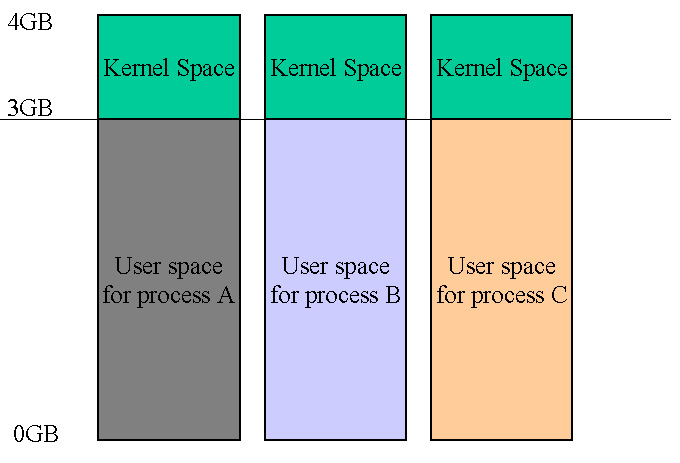
\includegraphics[scale=0.4]{img/user-kernel-space.jpg}
\end{figure}

\end{frame}


\section{Compiling the kernel}

\begin{frame}{Kernel configuration file}

\begin{figure}
  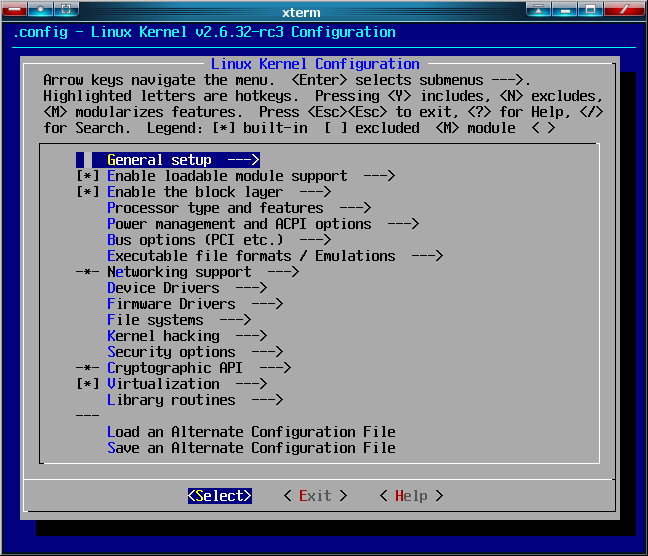
\includegraphics[scale=0.4]{img/Linux-kernel-menuconfig.png}
\end{figure}
\end{frame}


\begin{frame}{build targets}
\begin{itemize}
	\item {\bf config}, update config using a line oriented program
	\item {\bf i386_defconfig}, build for i386
	\item {\bf vmlinux}, builds the bare kernel image
	\item {\bf bzImage}, builds compressed kernel image
	\item {\bf modules}, builds all modules
	\item {\bf clean}, remove most generated files
\end{itemize}
\end{frame}

\begin{frame}{Compilation steps}
\begin{itemize}
	\item make menuconfig
	\item make bzImage
	\item make modules
	\item make modules_install
	\item create initial ramdisk
	\item update grub entry
	\item reboot
\end{itemize}
\end{frame}

\section{Kernel Modules}


\begin{frame}{Kernel modules}

\begin{itemize}
	\item {\bf printk}
	\item {\bf dmesg}, print or control the kernel ring buffer
	\item {\bf insmod}, insert a module into the kernel
	\item {\bf rmmod}, remove a module form the kernel
	\item {\bf modprobe}, add or remove modules
	\item {\bf modinfo}, show information about a module
\end{itemize}
\end{frame}

\begin{frame}[fragile]{Simple kernel module}
\begin{verbatim}#include <linux/kernel.h>
#include <linux/init.h>
#include <linux/module.h>

MODULE_DESCRIPTION("My kernel module");
MODULE_AUTHOR("Me");
MODULE_LICENSE("GPL");

static int simple_init(void)
{
        printk( KERN_DEBUG "Hi\n" );
        return 0;
}
static void simple_exit(void)
{
        printk( KERN_DEBUG "Bye\n" );
}
module_init(simple_init);
module_exit(simple_exit);                          
\end{verbatim}
\end{frame}

\begin{frame}[fragile]{Makefile}
\begin{verbatim}
KDIR=/lib/modules/`uname -r`/build
kbuild:
        make -C $(KDIR) M=`pwd`
clean:
        make -C $(KDIR) M=`pwd` clean
\end{verbatim}
\end{frame}




\begin{frame}[fragile]{Kbuild}
\begin{verbatim}
EXTRA_CFLAGS = -g
obj-m        = simple.o
\end{verbatim}
\end{frame}




\section{Keywords}

\begin{frame}{Keywords}
      \begin{itemize}
        \item make, kbuild
	\item insmod, rmmod
	\item bzImage, initrd
	\item built-in, loadable
      \end{itemize}
\end{frame}

\section{Questions}

\end{document}
